\documentclass[12pt]{extarticle}
\usepackage{listings}
\usepackage{graphicx}
\usepackage{float}
\usepackage{enumitem}
\usepackage{url}
\usepackage{hyperref}
\usepackage{titlesec}
\usepackage{eurosym}
\usepackage{subfiles}
\usepackage [autostyle, english = american]{csquotes}
\usepackage[top=2.75cm, bottom=1.75cm, left=1.75cm, right=1.75cm]{geometry} 
\usepackage{fancyhdr}
\usepackage{ragged2e}
\usepackage{graphicx}




\begin{document}

\begin{titlepage}
	\centering
	{\scshape\LARGE University of Idaho \par}
	\vspace{1cm}
	{\scshape\Large CS 383\par}
	\vspace{1.5cm}
	{\huge\bfseries Design Specification\par}
	\vspace{2cm}
	{\Large\itshape Trevor Morse\par}
	{\Large\itshape Peter Fetros\par}
	{\Large\itshape Zachary Spence\par}
	{\Large\itshape Matthew Holman\par}
	{\Large\itshape Domanic Welker\par}
	{\Large\itshape Adonay Berhe\par}
	\vfill
	supervised by\par
	Mr. Bruce \textsc{Bolden}
	
	\vfill
	
	% Bottom of the page
	{\large \today\par}
\end{titlepage}


\clearpage
\tableofcontents

\clearpage

\section{General}
This design spec is to outline and specify the details of our team's Tower of Light project. Throughout this document our team will detail how we have decided to develop this application, starting with our goals and getting down to functionality and features.  It will also detail the design decisions and adjustments made over time as the project has progressed.

\subsection{Goals}
The primary goal is the completion of our Tower of Light application by Thursday, December 15. This can be achieved through the completion of  each sprint such that it will result in a finished product.
	\begin{itemize}
		\item Our first goal was the completed design of our application. The original design specification was an integral portion of this goal.  Our mockups and design meetings were the other main portion.  This goal is the fundamental building block for the creation of the project.  As part of the goal, each team member developed a section of the design spec; following which, the team created editor and toolbox mockups and met in meetings to determine core functionality and extra features.
		\item Our second goal was the creation of working sections of the project: a working UI and a back-end IO.  The team split the UI into the editor portion and the toolbox portion, and determined the backend should run the data as well as IO.  Thus, the goal was to create a testable toolbox, a testable editor window, and a testable backend.  The focus was on core functionality, rather than expansions of the program.  The team wanted something that worked over something that had lots of potential.
		\item Our third and final goal was, once all core functions were complete, to include as many agreed-upon additional features as possible before the due date. The completion of this goal is equivalent to achieving our overall goal.  
	\end{itemize}
\subsection{Development Plans}
We went on to develop our application through the specified goals, modified as necessary over time, and time line for sprints, both as originally envisioned and as modified in class. Each week we set a task for each pair in the team to finish by the sprint deadline until the project is completed. Given time constraints, this will be a difficult process with multiple meetings to discuss the completion and feasibility of these weekly tasks. 
\subsection{Timeline}
This time line is a rough estimate of each week's tasks that will be completed to finish our Tower of Lights application. It has yet to be fully reviewed by the team and is subject to change.
	\begin{itemize}
		\item \textbf{Week 1 (10/26 - 11/2)} The first week was dedicated to completing the rough draft of this Design Specification. It was completed on time and in good order.
		\item \textbf{Week 2 (11/2 - 11/11)} Initial development: one pair began the toolbox development; a second pair began the editor development; and the final pair began the IO and data work.  Toolbox and editor should be in Qt's mockup language, QML.  This was completed on time and in good order.
		\item \textbf{Week 3 (11/11 - 11/18)} Continued development: User Interface was switch from mockups into a base form in the Qt project; while the backend code was to be in first completion.  Essentially, the goal was to be at the 5o percent completion mark.  This was completed on time and in fairly good order.  The editor window had posed some difficulty, but was overcome.
		\item \textbf{Week 4 (11/18 - 11/25)} Continued development: complete pieces.  Essentially, the goal here was to have the toolbox, backend, and editor in the 100 percent conmpletion.  This would allow the bringing together of all the pieces into one for the main prototype.  This goal was partially completed, though in good order.  The toolbox was about 95 percent complete, the backend data was 100 percent complete, and the editor was about 85 percent complete.  
		\item \textbf{Week 5 (11/25 - 12/2)} Continued development: finish the previous sprint and put the pieces into a prototype for presentation.  In this goal, both the toolbox and editor had to be finished as isolated windows and then integrated with the backend into the main project.  This goal was completed, and in good order.  
		\item \textbf{Week 6 (12/2 - 12/9)} Continued development: present prototype, bring all documentation up-to-date, and finaluze all core functions and additions as time permits.  One member of the editor pair was shifted to updating documentation, while the pair that finished the backend data took on the protoype and presentation.  Other members of the group took on modified coding assignments.  This goal was completed, and in good order.
		\item \textbf{Week 7 (12/9 - 12/15)} Finish development: Have a working version of the main program, run final testing, finish all documentation, craft all final memorandums, and turn in project.
	\end{itemize}


\clearpage
	\section{Editor}
	The editor is that part of the main window in which the frames and the frames' LED cells are displayed.  This editor window seeks to keep all the old functionality while adding improvements, such as an easier process for adding and deleting frames, and different navigational  processes.
	\subsection{Mock-up}
	\begin{figure}[!htb]
		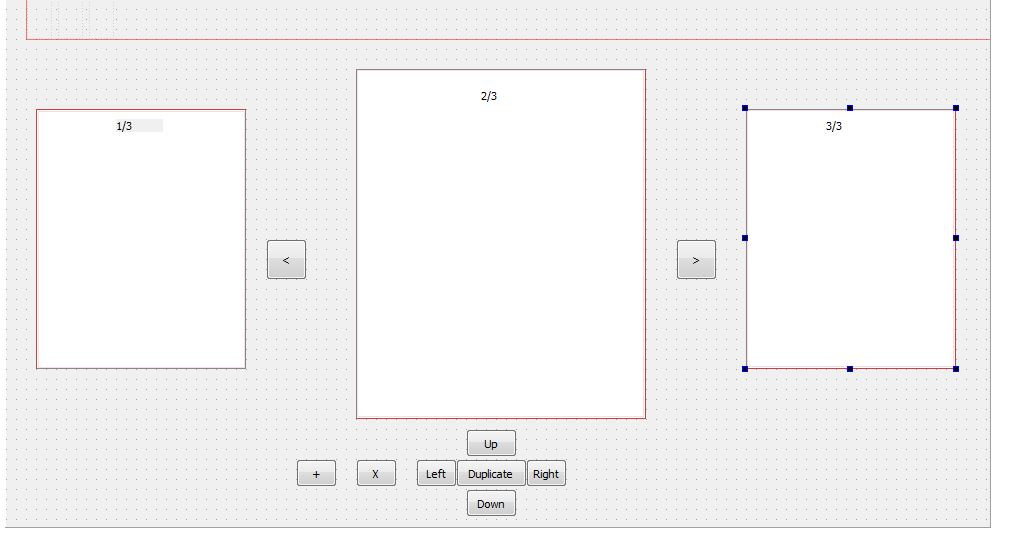
\includegraphics[width=\linewidth]{/Users/Zachary/tol/docs/design_spec/current_iteration_editor.jpg}
		\caption{Initial Mock-up of the editor section of the GUI.}
		\label{fig:editor_view}
	\end{figure}
	
	\subsection{Functionality}
	The following descriptions reference Figure \ref{fig:editor_view} above.
	\begin{itemize}
		\item This section of the GUI is the primary area for editing a frame within the overall animation. The primary focus is on the current frame in the center of the view, with smaller references to the previous and subsequent frames to the sides.  The premise behind this design choice is that with three visible frames in the main editing window, the user will be able to more easily craft animations that require multiple frames, such as doing a "w".  The user, with three immediately visible frames, will be able to view duplications and shifts more easily.
		\item Navigation:
		\begin{itemize}
			\item Above the current frame, there is an indicator of the current position relative to the total number of frames, allowing the user a better idea as to where each frame is in the animation.
			\item In order to navigate to a previous or subsequent slide, the user will click on the arrows to the sides of the current frame.  When one of these buttons is clicked, then it will shift the frames left or right, modifying the current view.  This creates a rotating list of frames for the user.
			\item Possible Addition: Mini-frame representations surrounding the numbers indicating the position of the frame. These could allow for speedy navigation across a large number of frames.  Essentially a list of thumbnails, this allows the user to click to the area of the animation as needed, rather than rotating all the way through with the left/right navigation buttons.
		\end{itemize}
		\item Editing:
		\begin{itemize}
			\item In order to edit a given frame, the user will utilize a combination of features in this section as well as in the toolboxes. (See Section toolbox for more details.)
			\item The current frame will be enlarged in the center of the view. Each panel inside represents an LED panel on the tower (panels in the figure are not necessarily to scale).  The panels are also only editable when in the current frame.  If in the previous or next frame, the user will be unable to edit them, preventing any slips on already finished or yet to be edited frames.  This also allows the user to focus on the current frame.
			\item The user will be able to select one or more LED panels at a time and specify the given options within the toolboxes.
			\item Below the current frame are a series of buttons. One allows the user to insert a new, blank frame immediately after the current frame. Another button allows the user to duplicate the current frame in a new frame after it.  The button with an "x" on it deletes the current frame.  The up/down/left/right labeled buttons are for the shifted duplications as used in the original tower lights animator.  Thus, maintaining the old functionality alongside new additions. 
		\end{itemize}
	\end{itemize}
	
	\subsection{Notes}
	\begin{itemize}
		\item The editor section of the GUI  works alongside the toolboxes. These toolboxes willl display to the left of the editor. They will provide options for editing a particular LED panel and/or overall frame. %TODO: reference the Toolbox section here
		\item There will also be options in the GUI's menus that will help with more efficient editing and navigation of frames.
		\item The development of the UI of the editor was one of the first to-do items determined by the team.  This was to help solidify the design before construction of the code itself. Once the design was solidified, more in-depth functionality was added.  This included working navigation, adding and deleting frames, etc.
	\end{itemize}
	
\clearpage
\section{ToolBox} \label{toolbox}
	
	\subsection{Functionality: General}
	The ToolBox portion of the GUI is a rectangular area that containing several different tabs. Each tab contains tools for a specific category.  On the first tab, tools used for color manipulation, editing, and other color tasks are housed.  And on the second tab, tools for editing, manipulating,and expanding frames of the animation are housed. These tabs are the “Color Tab” and the “Editing Tab” and are described below in more detail. However more tabs may be added as future improvements.
	\subsection{Functionality: Color Tab}
This tab will include several tools used for selecting and saving colors that will then be used for creating the tower lights animation frames. The following are the current features planned for this tab.
	\begin{itemize}
			\item Color pallete for visually selecting the desired color by using the mouse to click on a location within the pallete.  This allows the user to choose a color based on what he/she sees in his/her head.  It also does not require a user to be familiar with html-style hex, HSV, or RGB, which are other methods of selecting a color within this tab.  
			\item Predefined color selection box as well as a box to select colors that have previously been saved for easier access later.  This allows a user to not have to define common colors, like blue and red, and not to have redefine colors used througout the animation.  It also allows a user to have some colors to go back and forth between without having to use the pallete.
			\item Several  boxes that allows a text input representation of a color in the following format:
		\begin{itemize}
				\item Red, Green, Blue (RGB)
				\item HTML Hexadecimal Codes
				\item Hue, Saturation, and Value ( HSV )
				\item A future feature that could be added is Cyan, Yellow, Magenta, and Key ( CYMK )
		\end{itemize}
	\end{itemize}

	\subsection{Functionality: Editing Tab}
	This tab will include several tools used for selecting and editing frames that have already been made. This includes features such as
	\begin{itemize}
			\item Adding a range of frames: Insert a large number of frames by referring to the frame index and the number of frames you'd like to insert.  This allows the insertion of many frames without having to insert one frame at a time repeatedly.  This is especially useful when the user wants to insert arbitrarily many frames.
			\item Removing a range of frames: Remove a large number of frames by referring to the first and last frame indices that you would like to remove.  This allows the deletion of arbitrarily many frames, without having to delete one frame at a time repeatedly.  useful again, when the user wants to delete a large number of frames.
			\item Copying sections of a frame: Designate a frame and add its content to a selection of other frames.  This allows a user to reuse certain frames within an animation; especially useful when a user is reusing common themes, like letters or comets.
			\item Time Intervals: this allows a user to set the duration of time for a particular frame, and to view the current time for the frame being viewed.  The time intervals are in milliseconds, which allows easier usage by the user.
	\end{itemize}

	\subsection{Functionality: Music Tab }
	This tab will allow the user to specify a music file and commit it to the animation.
	\begin{itemize}
		\item A text box allows the user to type in the file name of the music file that the user wishes to use.  
		\item A button named "Commit" allows the user to commit the specified file to the animation.  The backend for this runs some checks to make sure the file is of the proper type.
	\end{itemize}

	
	\subsection{Notes}
	\begin{itemize}
		\item The toolbox section of the GUI works alongside the Editor section to create a frame/animation. 

		\item It will be possible to later designate more ToolBox Tabs such that Tabs can be added and removed at will by both programmers and users.
	\end{itemize}


\clearpage
\section{Menu Bar}



\subsection{Introduction}

{This specification document illustrates the base features of the intended Menu bar of the new Tower of Lights editor. The bar contains numerous features that are similarto the existing UI with a few additions. The descriptions of the sections are listed as follows.}

\subsection{Features and Descriptions}

\begin{itemize}
\item \textbf{File}

{This drop-down list deals with IO manipulation. Features include:}

	\begin{itemize}
	\item \textbf{New} - Creates a new blank project. Currently, the frames are loaded with a single start, so this is a future improvement.
	\item \textbf{Open} - Opens an existing .tan2 file for editing.
	\item \textbf{Save} - Saves file.
	\item \textbf{Save As} - Similar to traditional "Save As" option.  This is not a core feature, but could be implemented.
	\item \textbf{Close} - Closes window.   This is not core functionality, and would be added if time allows.  The window already has a close button provided, which renders this a convenience.


	\end{itemize}


\end{itemize}

\subsection{Future Works}

{These features will not be present in the first few iterations of the software; however, if time permits should be implemented.  The playback features are important features that are, if not core functionality, a must for additional functionality. }

\begin{itemize}

\item \textbf{Edit}

{This drop-down list displays options for editing the document at a frame-level (rearrange, delete, insert, clear, ...) and cell-level (individual box). For some of these functionalities - Insert, Delete, Copy ... - short-cut icons will be available on the editor window.  This section is also not required core functionality.  As much of it is implemented elsewhere, and what is not is also additional features.  Therefore, this will only be added if time permits.}

	\begin{itemize}
	\item \textbf{Insert} - Insert a frame before or after current frame.
	\item \textbf{Delete} - Delete current frame.
	\item \textbf{Clear} - Clear entire frame.
	\item \textbf{Clear Cell} - Clear LED selection of a specific cell.
	\item \textbf{Randomize} - Fill a frame with random combinations of colors and shades.
	\end{itemize}

\item \textbf{Tools}

{This drop-down list will include all the tool-boxes that the editor will be using including a checkbox option for users to check-off tools that they desire to have present in the editor window. Tool boxes include:}

	\begin{itemize}
	\item \textbf{Frame toolbox}
	\item \textbf{LED toolbox}

	\end{itemize}

\item \textbf{Search}

{This option will enable users to search for a specific frame by label or frame number.  Again, this is an additional feature to be added as time permits.}

\item \textbf{Playback}

{This drop-down list will be used to play, pause, or stop the various animations created within an open file. Options include: }
	\begin{itemize}
	\item \textbf{Play/Pause} - Play or pause an animation.
	\item \textbf{Stop} - Stops an animation and resets frame location to the beginning.
	\item \textbf{Preview Mode} -Plays animation in a new window with pictorial representation of the Tower building.

	\end{itemize}

\item \textbf{Animations}

{This feature will be added under "Edit". The purpose of this feature is to enable users to select from a list of built-in animations (snake, sine wave, ...) and specify the number of frames to be used upon creation of animations. Due to lack of time and presence of features with higher-priorities, implementation of this feature will take place in the very late stages of development, as time permits. }

\end{itemize}

\clearpage
\section{Additional Features/ Potential Improvements}
{There are a variety of additional features and potential improvements that we believe can be made to the basic functionality demonstrated in both versions 1 and 2 of the tower lights design program. The first of the following improvements are ranked first by the number of times they were mentioned in the design meeting, with the most often mentioned features ranked first and descending from there. Please note that after the first few entries, the features are essentially unranked as they were each only mentioned once and thus have equal weighting in the list.}

\begin{itemize}
	\item Clear Frame (Four Mentions)
	\begin{itemize}
		\item The user should be able to clear the contents of a frame either by clicking a button, pressing the `del' key, etc.
	\end{itemize}
	\item Multi-Selection/ Editing (Three Mentions)
	\begin{itemize}
		\item The user should be able to select multiple frames, perhaps click + shift key, banding box, etc. and then edit those frames by changing their location in the animation, clearing their contents, etc.
	\end{itemize}
	\item Predefined Animations (Three Mentions)
	\begin{itemize}
		\item A series of predefined animations (comets, raindrops, snake effect, text, etc) should be available to insert into the final set of frames and will be able to last a specified duration.
	\end{itemize}
	\item Random Frame Generator/ Animation Generator (Three Mentions)
	\begin{itemize}
		\item With the click of a button, the user should be able to generate random color values in either a single frame, or over multiple frames.
	\end{itemize}
	\item Playback Preview (Two Mentions)
	\begin{itemize}
		\item A dedicated view/ window displays the playback of the frames as it would appear on the actual tower. This feature could possibly include playback of the music as well, in conjunction with the changing color values so that the entire effect can be previewed.
	\end{itemize}
	\item Adjust Position of Frames (Two Mentions)
	\begin{itemize}
		\item The user should be able to move an existing frame from one part of the animation to another without having to redraw the entire frame from scratch.
	\end{itemize}
	\item Auto-Import Time Codes Based on Music (Two Mentions)
	\begin{itemize}
		\item When a user selects a song, generate a number of empty frames in the animation based on the length/ tempo of the song.
	\end{itemize}
	\item Window Scaling (One Mention)
	\begin{itemize}
		\item When the user resizes the window, perhaps to a fullscreen view, the various tools/ views, etc. should scale appropriately.
	\end{itemize}
	\item Time Units (One Mention)
	\begin{itemize}
		\item Time codes for frames can be generated based on the particular tempo of a song for a set duration. For example, one section could have one frame per beat for sixteen beats at a speed of 120 beats per minute, then another section immediately following that one might have twenty beats at a speed of 136 beats per minute.
	\end{itemize}
	\item Customizable Defaults (One Mention)
	\begin{itemize}
		\item If there is a particular workflow/ layout/ set of color choices etc. that a user uses, those choices should be able to be saved and used again for a later project.
	\end{itemize}
	\item Scrollable Context (One Mention)
	\begin{itemize}
		\item The frames of the animation should be visible and the user should be able to scroll through them all.
	\end{itemize}
	\item Save Custom Colors (One Mention)
	\begin{itemize}
		\item The user should be able to save a specified color to a color palette for use later in the animation process. This was implemented as part of the toolbox.
	\end{itemize}
	\item Move Tower Indicator Box/ Snapshot Button $\rightarrow$ Frame (One Mention)
	\begin{itemize}
		\item Currently, in the second version of the tower of lights project, there is a design window where the user can enter information outside a `view frame' that will be used to generate the individual frames of animation. Currently, the view frame is static and the information around it moves in relation to the static frame. This leads to information loss when the user moves the information too far to the edges. By moving the view frame and having the user click a `snapshot' button to confirm that data that should be written to the animation frame, this data loss is mitigated.
	\end{itemize}
	\item Arrow Keys $\rightarrow$ Duplicate Frame (One Mention)
	\begin{itemize}
		\item Similar to how the directional buttons on the second version of the tower of lights project function, now the user should be able to use the arrow keys to get the same functionality.
	\end{itemize}
	\item Shortcuts to Adjust LED Settings (One Mention)
	\begin{itemize}
		\item The color/ brightness of the LEDs should be adjustable quickly and easily.
	\end{itemize}
	\item Zoom View of Design Panel (One Mention)
	\begin{itemize}
		\item The user should be able to zoom in and out of the design panel, similar to the one implemented in version two of the original tower of lights project, to see more or less of the surrounding information that the frame can utilize for animations. 
	\end{itemize}
	\item Auto-Save User Progress (One Mention)
	\begin{itemize}
		\item Automatically save the users work every so often - just in case the program crashes.
	\end{itemize}

\end{itemize}

\clearpage

\section{Output of Program}
The output required of this program, in order for it to interact with the current system, must be in the .tan2 format.  This format has three major pieces: the header, the frames, and the time signatures.
\newline
\subsection{Header for the .tan2 File}
The header is divided into 5 pieces:
	\begin{itemize}
		\item The Version Number: 0.4 in the current, perhaps 0.5 or 1.0 for this project
		\item File Type: either NoAudioFile or its converse--i.e., the audio file associated with the .tan2
		\item Last Color Used: the last RGB value used in editing the frames
		\item List of Pre-Set Colors: the RGB values for each of the pre-set colors included in the program
		\item Show information: the number of frames, the heighth, and the width of the tower in the frame
	\end{itemize}
\subsection{Frames in the .tan2 File}
The frames are displayed in a particular format in the .tan2 file.
	\begin{itemize}
		\item It is essentially a grid of numbers, from 0 to 255
		\item Each group of 3, reading from left to right, represents the color of 1 LED in the frame
		\item There is a color for each of the LEDs in the frame, not just the 10x4 that is the actual tower windows
	\end{itemize}

\subsection{Time Signatures}
The start value, usually 0, is placed directly after the header and before the first frame.  After each of the frames is the next time signature, which is the previous value plus the increment specified by the editor.  The exception is the final frame, which is not followed by a time signature, and terminates the file.  The default is .050 s, which shows up as 50 in the .tan2 file.  Hence the default measure of time in the program is ms.

\subsection{File Example}

0.4  \\
NoAudioFile\\
0 0 255 \\
169 169 169 128 128 0 139 0 139 0 139 139 0 0 139 0 100 0 139 0 0 0 0 0 128 128 128 255 255 0 255 0 255 0 255 255 0 0 255 0 128 0 255 0 0 255 255 255 \\
1 10 4 \\
0 \\
0 0 0 0 0 0 0 0 0 0 0 0 0 0 0 0 0 0 0 0 0 0 0 0 0 0 0 0 0 0 0 0 0 0 0 0 \\
0 0 0 0 0 0 0 0 0 0 0 0 0 0 0 0 0 0 0 0 0 0 0 0 0 0 0 0 0 0 0 0 0 0 0 0 \\
0 0 0 0 0 0 0 0 0 0 0 0 0 0 0 0 0 0 0 0 0 0 0 0 0 0 0 0 0 0 0 0 0 0 0 0 \\
0 0 0 0 0 0 0 0 0 0 0 0 0 0 0 0 0 0 0 0 0 0 0 0 0 0 0 0 0 0 0 0 0 0 0 0 \\
0 0 0 0 0 0 0 0 0 0 0 0 0 0 0 0 0 0 0 0 0 0 0 0 0 0 0 0 0 0 0 0 0 0 0 0 \\
0 0 0 0 0 0 0 0 0 0 0 0 0 0 0 0 0 0 0 0 0 0 0 0 0 0 0 0 0 0 0 0 0 0 0 0 \\
0 0 0 0 0 0 0 0 0 0 0 0 0 0 0 0 0 0 0 0 0 0 0 0 0 0 0 0 0 0 0 0 0 0 0 0 \\
0 0 0 0 0 0 0 0 0 0 0 0 0 0 255 0 0 255 0 0 255 0 0 255 0 0 0 0 0 0 0 0 0 0 0 0\\ 
0 0 0 0 0 0 0 0 0 0 0 0 0 0 255 0 0 0 0 0 0 0 0 255 0 0 0 0 0 0 0 0 0 0 0 0 \\
0 0 0 0 0 0 0 0 0 0 0 0 0 0 255 0 0 255 0 0 255 0 0 255 0 0 0 0 0 0 0 0 0 0 0 0\\ 
0 0 0 0 0 0 0 0 0 0 0 0 0 0 255 0 0 255 0 0 0 0 0 0 0 0 0 0 0 0 0 0 0 0 0 0 \\
0 0 0 0 0 0 0 0 0 0 0 0 0 0 255 0 0 0 0 0 255 0 0 0 0 0 0 0 0 0 0 0 0 0 0 0 \\
0 0 0 0 0 0 0 0 0 0 0 0 0 0 255 0 0 0 0 0 0 0 0 255 0 0 0 0 0 0 0 0 0 0 0 0 \\
0 0 0 0 0 0 0 0 0 0 0 0 0 0 0 0 0 0 0 0 0 0 0 0 0 0 0 0 0 0 0 0 0 0 0 0 \\
0 0 0 0 0 0 0 0 0 0 0 0 0 0 0 0 0 0 0 0 0 0 0 0 0 0 0 0 0 0 0 0 0 0 0 0 \\
0 0 0 0 0 0 0 0 0 0 0 0 0 0 0 0 0 0 0 0 0 0 0 0 0 0 0 0 0 0 0 0 0 0 0 0 \\
0 0 0 0 0 0 0 0 0 0 0 0 0 0 0 0 0 0 0 0 0 0 0 0 0 0 0 0 0 0 0 0 0 0 0 0 \\
0 0 0 0 0 0 0 0 0 0 0 0 0 0 0 0 0 0 0 0 0 0 0 0 0 0 0 0 0 0 0 0 0 0 0 0 \\
0 0 0 0 0 0 0 0 0 0 0 0 0 0 0 0 0 0 0 0 0 0 0 0 0 0 0 0 0 0 0 0 0 0 0 0 \\
0 0 0 0 0 0 0 0 0 0 0 0 0 0 0 0 0 0 0 0 0 0 0 0 0 0 0 0 0 0 0 0 0 0 0 0 \\\\

In this example, the first line is the version number.  The second line is the file type; third line is the last color used; while the fourth and fifth lines are the pre-set colors.  The sixth line is the number of frames, the height of the tower, and the width of the tower.  The seventh line is the time signature; and the remainder is the grid of LED colors.

\subsection{Notes}
The format of the .tan2 file is very straightforward.  It has simple requirements, and these could be easily produced.  The data required would also be fairly easy to store, as both the pre-set colors and the grid of LEDs could be stored in arrays, while the type and the last color used could be variables.  The version number and tower size could be constants.  And the time signatures could be determined as the frames are added on; while the frame number could be the size of a linked list holding the frames.  

\end{document}
